\bbsection{Database Schema}{database-schema}

\bbsubsection{Core Data Diagram}{core-data-diagram}
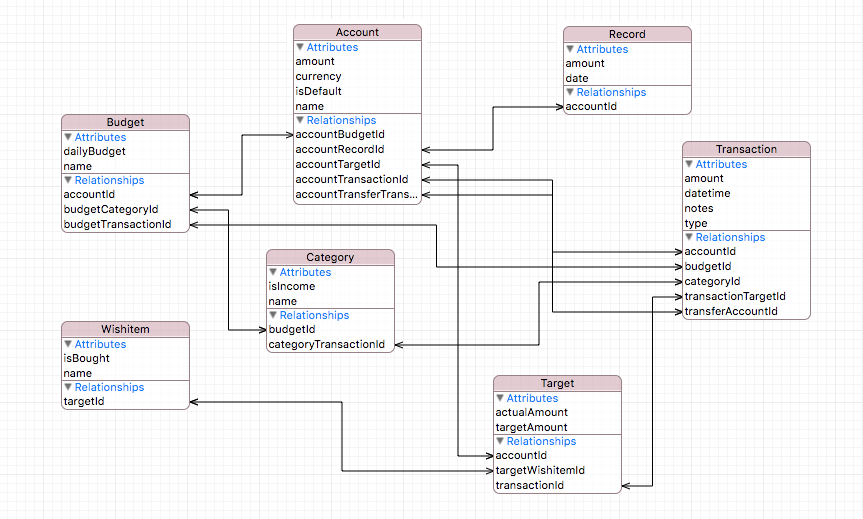
\includegraphics[scale=0.55]{core-data}

\bbsubsection{Model Attributes}{model-attributes}

\bbsubsubsection{Account}{account-attributes}
\begin{itemize}
\coreitem{amount}{double}{Contains the current amount present in the account.}
\coreitem{currency}{string}{Contains the country identifier for the currency used in the account.}
\coreitem{isDefault}{boolean}{If this value is true, then the account is the default account to use for everyday transactions.}
\coreitem{name}{string}{The name of the account.}
\end{itemize}

\bbsubsection{Model Relationships}{model-relationships}

\bbsubsubsection{Account}{account-relationships}
\begin{itemize}
\coreitem{accountBudgetId}{links with the Budget table}{Description to follow once implemented.}
\coreitem{accountRecordId}{links with the Record table}{Description to follow once implemented.}
\coreitem{accountTargetId}{links with the Target table}{Description to follow once implemented.}
\coreitem{accountTransactionId}{links with the Transaction table}{Description to follow once implemented.}
\coreitem{accountTransferTransactionId}{links with the Transaction table}{Description to follow once implemented.}
\end{itemize}